\scanpage{79}
\diagram{\begin{tikzcd}[ampersand replacement=\&]
0\arrow[r]\&E'(A)\arrow[r]\arrow[d,"\unsure{2|?}"]\&E(A)\arrow[r]\arrow[d,no head]\&E(K)\arrow[r]\arrow[d,no head]\&0\\
0\arrow[r]\&\sum\unsure{E^d|E'}(\hat A_p)\arrow[r]\&\sum E(\hat A_p)\arrow[r]\&\sum E(K_p)\arrow[r,no head]\&0
\end{tikzcd}}

\diagram{\begin{tikzcd}[ampersand replacement=\&,column sep=large]
\&\begin{array}{l}\operatorname{Pic}(A)/2\operatorname{Pic}(A)\subset H^2(A,\mu_2)\end{array}\arrow[d,phantom,"\unsure{\Vert|\wr}" description]\&\&E(K)\arrow[d,equal]\\
0\arrow[r]\&F'(A)\arrow[r]\&F(A)\arrow[r,no head]\arrow[d]\&F(K)\arrow[d]\&\deleted{\unsure{\text{---}}}\\
\&0\arrow[r]\&\sum F(\hat A_p)\arrow[r,"\text{inj}"']\&\sum F(K_p)
\end{tikzcd}}
\margin{A anneau de Dedekind ----}

\deleted{\figure{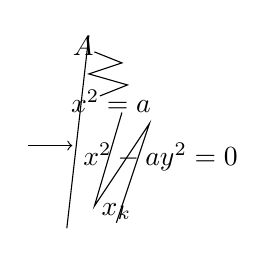
\begin{tikzpicture}[x=.7cm,y=.7cm]
\node at (0,3){$A$};\node at (.5,2){$x^2=\unsure{a}$};
\node at (1.4,1){$\unsure{x^2}-ay^2=0$};\node at (.6,0){$\unsure{x_k}$};
\draw[->](-1,1.2)--(-.2,1.2);\draw(.1,3.2)--(-.3,-.3);
\draw(.2,2.9)--(.7,2.7)--(.1,2.5)--(.8,2.3)--(.3,2.1);
\draw(.7,1.8)--(.2,.1)--(1.2,1.6)--(.6,-.2);
\end{tikzpicture}}}

\margin{$\unsure{\mathbb Q|\mathbb Z}/2\mathbb Z$}
\deleted{\diagram{\begin{tikzcd}[ampersand replacement=\&]
H^1(A,\mathbb Z/2\mathbb Z)\arrow[r]\&\sum_pH^1(\hat A_p,\mathbb Z/2\mathbb Z)\\
H^1(K,\unsure{G_m|\mathbf G_m})\arrow[r]\&{}
\end{tikzcd}}}
\deleted{\diagram{\begin{tikzcd}[ampersand replacement=\&]
0\arrow[r]\&T\arrow[r]\&JT\arrow[r]\&\unsure{MT|M_T}\arrow[r,no head]\&0\\
\unsure{K} \&0\arrow[r,no head]\&L^*\arrow[r]\&J_L\arrow[r,no head]\&C_L\arrow[r,no head]\&0\\
\&0\arrow[r,no head]\&L^*\otimes X\arrow[r,no head]\&J_L\otimes X\arrow[r,no head]\&C_L\otimes X\arrow[r]\&0
\end{tikzcd}}}
\deleted{\[
\unsure{H^1}\qquad H^{\unsure{1}}(G,\ \longrightarrow\ H^{\unsure{1}}(
\]}
\deleted{\[
\sum_pH^1(G_p,\unsure{L_p^*|K_p^*}\otimes X)\longrightarrow
\]}
\deleted{\[
H^{\unsure{1}}(G,K^*)\longrightarrow H^{\unsure{1}}(G,J)
\]}

$\unsure{E'|E^d}(V)$ \inserted{\diagram{\begin{tikzcd}[ampersand replacement=\&,column sep=small,row sep=small]\&\begin{array}{l}\text{anneau de val. discrète}\\\text{complet}\end{array}\\\phantom{V}\arrow[ur,bend left=22]\end{tikzcd}}} est isomorphe à la somme directe d’une infinité de copies de $\unsure{F(k)|E(k)}$, avec $k$ le corps résiduel
\margin{78}
